\chapter{Evaluation}

\label{Evaluation} % For referencing the chapter elsewhere, use \ref{Chapter1}

The Evaluation chapter is structured into three main sections, 
systematically analyzing the components crucial for a transformer embedding based malware detection system 
(Figure \ref{fig:bertbased_malwaredetection_schema}). 
First, the APK Representation section \ref{sec:apkrepresentation} evaluates the impact of different APK feature combinations extracted 
from Android manifest files on malware classification performance, using ModernBERT embeddings with frozen parameters. 
Next, the Transformer Encoder section \ref{sec:tran_enc} explores the performance implications of unfreezing encoder parameters during training, 
comparing ModernBERT against other transformer variants like BigBird and Longformer, 
and analyzing their impact on model performance across different APK representations. 
Lastly, the Decision Head section \ref{sec:decision_head} investigates various decision head strategies, 
including averaging embeddings and using DetectBERT, and assesses their effectiveness in classifying APK representations 
when exceeding the encoders context windows.

\section{The APK Representation}
\label{sec:apkrepresentation}

\begin{marginfigure}[3\baselineskip] % move figure up by 1 line -5\baselineskip
    \center
    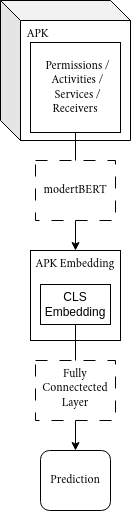
\includegraphics[width=0.6\marginparwidth]{4_Evaluation/permission_transformer_schema.png}
    \caption{\label{fig:permission_transformer_schema}
    Distribution of malware and goodware samples across datasets shown as pie charts.
    The datasets analyzed are are ordered by size from largest to smallest.
    The number of APKs contained in the Dataset are shown in brackets}
\end{marginfigure}

%Intro
A crucial factor in designing a transformer embedding-based mobile malware detection system is how the APK is represented. 
Since most embedding models, including all the BERT models considered, cannot process an APK in its entirety, 
specific features, such as permissions, API calls, or manifest attributes, must be selected and formatted in a tokenizable manner. 
To ensure reliable comparisons across different APKs, these features should be structured consistently.

%How a representation is build
To organize these features effectively, 
it is useful to concatenate them using designated tokenizer vocabulary entries as separators.
In this study, a varying number of \# characters were used as separators. 
Different separators were applied to distinguish between various types of separations, 
such as separating feature categories and distinguishing elements within a feature list.

%Setup of first experiment
To demonstrate how different APK representations affect the performance of a malware detection architecture, 
an experiment was conducted using a relatively simple stack, as shown in Figure \ref{fig:permission_transformer_schema}.
To isolate the impact of representation, the other two variables in the stack were kept static. 
For simplicity and efficiency, ModernBERT \cite{modernbert} was selected as the embedder. 
Since ModernBERT supports a context window of up to 8000 tokens, each APK could be processed in a single iteration, 
ensuring that the entire representation was captured in one pass. 
This approach showed good efficiency by reducing computational overhead while preserving relationships within 
the extracted APK features.
The embedding size was set to 768, as recommended by the original ModernBERT authors. 
After embedding, each input token, along with a blank CLS token, was represented by 768 floatingpoint values. 
Once each APK was embedded, a simple fully connected layer with dropout was trained for five epochs  
on the time based split subset of the dataset, as described in the previous chapter. 
To simplify processing, the decision head was not trained on the full embedding but only on the CLS token embedding. 
As a result, each APK was represented by 768 floatingpoint values, 
ensuring a compact yet informative representation for classification.
During training, only the weights of the final fully connected layer were updated, 
while the weights of the ModernBERT embedder remained frozen. 
The fully connected layer was chosen for its simplicity and effectiveness in classification tasks, 
while the dropout mechanism was included to prevent overfitting and improve generalization.
With this setup, multiple APK representations could be explored. 
However, each representation was constrained to 8000 tokens to ensure compatibility with 
ModernBERTs processing window. 
The selected representations were all extracted from the AndroidManifest.xml file, 
which contains essential metadata about an application's permissions, activities, services, and receivers. 
These components are often indicative of an applications behavior and potential security risks \cite{malbert}.
The chosen representations included the names of the permissions requested by the APK, 
the names of the marked activity java classes, and the names of the marked service and receiver classes. 
Permissions indicate which resources an application can access, 
while activities, services, and receivers provide insight into its execution behavior.

\begin{table}[b!]
    \caption{\label{tab:apk_representation_results}%
    Performance of different APK representations using frozen ModernBERT embeddings. Features are extracted from Android manifest.xml (A=Activities, P=Permissions, R=Receivers, S=Services). Results reported on time-based transcend subset split after five epochs.}
    \resizebox{\textwidth}{!}{%
    \begin{tabular}{@{}lcccc@{}}
    \toprule
    \textbf{Representation} & \textbf{Accuracy} & \textbf{Precision} & \textbf{Recall} & \textbf{F1} \\ 
    \cmidrule(r){1-1} \cmidrule(lr){2-5}
    A + P + R + S & 74.45\% & 76.30\% & 70.58\% & 73.33\% \\
    A + P + S      & 74.67\% & 76.39\% & 71.09\% & 73.64\% \\
    A + P          & 74.47\% & 74.10\% & 74.89\% & 74.49\% \\
    R + S          & 65.12\% & 74.12\% & 45.97\% & 56.75\% \\
    A              & 70.64\% & 70.88\% & 69.62\% & 70.24\% \\
    P              & 66.51\% & 63.48\% & 77.01\% & 69.60\% \\
    S              & 65.12\% & 69.28\% & 53.77\% & 60.55\% \\
    R              & 50.23\% & 0.00\%  & 0.00\%  & 0.00\%  \\
    \bottomrule
    \end{tabular}%
    }
\end{table}

% Evaluation of Experiment 1
The performance results in Table \ref{tab:apk_representation_results} 
show how different representations of an APK affect malware detection. 
The combination of activities, permissions, receivers, and services (A + P + R + S) achieved an F1 score of 73.33\%, 
indicating that a comprehensive manifest representation is beneficial. 
However, excluding receivers (A + P + S) slightly improved performance to 73.64\%, 
suggesting that receivers introduce noise, which can negatively impact overall performance.
A subset containing only activities and permissions (A + P) achieved the highest F1 score of 74.49\%, 
confirming that these two features effectively capture essential malicious behaviors. 
Permissions alone (P) demonstrated high recall at 77.01\% but had lower precision at 63.48\%, 
highlighting their widespread use in both benign and malicious applications. 
Activities (A) provided a balanced performance with an F1 score of 70.24\%, 
emphasizing their significance in malware detection.

% negative impact of receivers
Including receivers (R) significantly degraded performance, 
leading to an F1 score of 0.00\% when used alone and reducing overall effectiveness when combined with other features. 
This result indicates that the model consistently predicts goodware, 
suggesting that receivers do not provide a reliable representation of malicious APKs. 
Services (S) also struggled, achieving an F1 score of 60.55\%, 
which implies that while these background components are relevant, 
they lack strong discriminative power when used in isolation.

% Comparison with decision tree
Comparing the results of this experiment, which uses permissions as the feature representation, 
with previous malware detection results based on a decision tree using only permissions 
(Table \ref{tab:decisiontreepermissions}) highlights the potential of this architecture. 
The improved performance suggests that this approach is highly promising, 
possibly due in part to the analysis of custom permission naming. 
However, it is important to note that the two experiments are based on different datasets. 
The decision tree experiment was conducted on the full Transcend dataset, 
while this experiment was performed on only a subset of it. 
In the next section, we demonstrate how performance varies between the full Transcend dataset and its subset.

\section{The Transformer Encoder}
\label{sec:tran_enc}

\begin{table}[b!]
    \caption{\label{tab:apk_representation_results_unfrozen}%
    Performance of different APK representations using \emph{unfrozen} ModernBERT embeddings. Features are extracted from the Android manifest.xml (A=Activities, P=Permissions, R=Receivers, S=Services). The encoder was also trained through backpropagation in this experiment.}
    \resizebox{\textwidth}{!}{%
    \begin{tabular}{@{}lcccc@{}}
    \toprule
    \textbf{Representation} & \textbf{Accuracy} & \textbf{Precision} & \textbf{Recall} & \textbf{F1} \\ 
    \cmidrule(r){1-1} \cmidrule(lr){2-5}
    A + P + R + S & 83.95\% & 88.67\% & 77.67\% & 82.81\% \\
    A + P + S     & 84.32\% & 85.14\% & 82.99\% & 84.05\% \\
    A + P         & 85.66\% & 87.88\% & 82.58\% & 85.15\% \\
    R + S         & 71.04\% & 87.89\% & 48.51\% & 62.51\% \\
    A             & 80.29\% & 90.22\% & 67.75\% & 77.39\% \\
    P             & 74.97\% & 72.20\% & 80.86\% & 76.28\% \\
    S             & 72.23\% & 88.46\% & 50.84\% & 64.57\% \\
    R             & 50.23\% & 0.00\%  & 0.00\%  & 0.00\%  \\
    \bottomrule
    \end{tabular}%
    }
\end{table}

% Intro
The second variable analyzed in the architecture for APK classification (Figure \ref{fig:bertbased_malwaredetection_schema}) 
is the Transformer Encoder.
In theory, several Transformer Encoders could be used in this approach, 
including BigBird \cite{bigbird}, Longformer \cite{longformer}, Performer \cite{performer}, 
Linformer \cite{linformer}, Reformer \cite{reformer}, FNet \cite{fnet}, Nyströformer \cite{nystromformer}, 
and DexBert \cite{dexbert}.
Before any of these encoders can process a representation of an APK, the input must first be tokenized.
Tokenization requires a vocabulary that maps different language pieces to tokens.
This vocabulary is learned during the training of an encoder model and is specific to each model.
In this work, preprocessing all APK representations by tokenizing them before encoding improved pipeline efficiency 
(e.g., Figure \ref{fig:permission_transformer_schema}).
This approach helped prevent queues of mixed GPU and CPU usage, optimizing the overall process.
However, this approach has a downside: backpropagation cannot be applied to the encoder model during training.

% Purpose of Transformer Encoder 
Once the APK representation is tokenized, the primary goal of the Encoder is to reduce its volume to a more manageable 
level while retaining all relevant information needed for classification.
Models with a large context window are particularly well suited for this task.
ModernBERT \cite{modernbert}, with its context window of up to 8000 tokens, is an especially promising candidate.
The Encoder produces an embedding of the APK representation, where the embedding size is a hyperparameter of the model.
For ModernBERT, the default embedding size is 768, this hyperparameter was kept static during all experiments of this thesis.

% Training Encoder experiment
The first experiment in this thesis that examines the Encoders effect on overall model performance 
is based on the same framework as the previous experiment (Figure \ref{fig:permission_transformer_schema}).
The only change in this setup was unfreezing the Encoder models parameters during training, 
allowing ModernBERT to refine its embeddings throughout the process.
The results of this modification are shown in Table \ref{tab:apk_representation_results_unfrozen}.
Comparing these results with those from the previous experiment, where the Encoder was frozen 
(Table \ref{tab:apk_representation_results}), reveals a performance increase in nearly every instance.
For receivers as a representation, the F1 score remained at 0\%, 
demonstrating that an improved Encoder cannot compensate for a fundamentally weak representation.
Apart from this case, performance improved across all other representations, 
with F1 score gains exceeding 10 percentage points in some cases.
More complex and combined representations saw the most significant improvements.
The F1 score of 85.15\% for the activities and permissions representation 
shows the potential of this simple yet efficient approach.

\begin{margintable}[-5\baselineskip]
    \caption{\label{tab:full_transcendence_permissions_a_p} Performance of Activities (A) and Permissions (P) as representations using the full transcending dataset and otherwise the same setup as for table \ref{tab:apk_representation_results_unfrozen}}
    \footnotesize
    \begin{tabular*}{\linewidth}{@{\extracolsep{\fill}} cccc@{}}
        \toprule
        \textbf{Acc.} & \textbf{Prec.} & \textbf{Rec.} & \textbf{F1} \\
        \midrule
        92.57\% & 67.97\% & 67.52\% & 67.74\% \\
        \bottomrule
    \end{tabular*}
\end{margintable}

\begin{margintable}[5\baselineskip]
    \caption{\label{tab:full_transcendence_permissions_a_p_s} Performance of Activities (A), Permissions (P) and Services (S) as representations using the full transcending dataset and otherwise the same setup as for table \ref{tab:apk_representation_results_unfrozen}}
    \footnotesize
    \begin{tabular*}{\linewidth}{@{\extracolsep{\fill}} cccc@{}}
        \toprule
        \textbf{Acc.} & \textbf{Prec.} & \textbf{Rec.} & \textbf{F1} \\
        \midrule
        92.33\% & 67.07\% & 65.98\% & 66.52\% \\
        \bottomrule
    \end{tabular*}
\end{margintable}

% Reduced performance on Full Dataset
Given the promising results of the basic algorithm, which embeds only the most fundamental APK features, 
another experiment was conducted using the full Transcend dataset.
Since A+P and A+P+S representations performed best, they were selected for this experiment.
Due to computational and time constraints, not all algorithms were tested on the full dataset.
Tables \ref{tab:full_transcendence_permissions_a_p} and \ref{tab:full_transcendence_permissions_a_p_s} 
present the results achieved on the full dataset.
While accuracy improved from approximately 85\% to 92\%, precision, recall, and F1 scores dropped by around 20 percentage points.
The higher accuracy indicates that the algorithm correctly classified both malware and goodware samples more frequently.
However, the decline in precision and recall suggests that the algorithm 
struggled more with detecting malware samples in this dataset.
This difference in performance can be attributed to the label class imbalance.
In previous experiments, the dataset had a balanced 1:1 malware-to-goodware ratio, whereas in the full Transcend dataset, 
only 11.6\% of the samples are malware, while 88.4\% are goodware.
These results suggest that the algorithms effectiveness in malware detection decreases when labels are unevenly distributed.
This finding underscores the importance of dataset size and balance in training 
transformer based models for Android malware detection.

% Work still has meaning
Comparing these results with those in Table \ref{tab:apk_representation_results_unfrozen} shows that using the 
full dataset leads to a decrease in performance.
However, the key conclusion from the previous experiment remains valid: the A+P representation continues 
to outperform the A+P+S representation.
While these results are not directly comparable to other algorithms benchmarked on the Transcend dataset, 
the insights gained from these experiments remain valuable.

% Setup Encoder switch experiment
Another experiment was conducted to assess the effect of changing the 
base model of the Transformer Encoder in the malware detection architecture.
For this, APKs were represented using their permissions and activities, 
and the same Transcend subset was used as in previous experiments 
(Tables \ref{tab:apk_representation_results} and \ref{tab:apk_representation_results_unfrozen}).
With the same general setup, three different Encoder base models were compared while training 
the Encoder alongside the decision head.
The models considered in this experiment were ModernBERT \cite{modernbert}, BigBird \cite{bigbird}, 
and Longformer \cite{longformer}.
These models were chosen for their reported simplicity, efficiency, 
and large context window sizes of 4000 and 8000 tokens, respectively.

% Results of Encoder switch experiment
Using the same approach as before, where the CLS token embedding serves as the input for the decision head, 
the performance of the models is shown in Table \ref{tab:encoder_model_comparison_cls}.
The results for both BigBird and Longformer are unsatisfactory, despite differences in their F1 scores.
In both cases, the models tend to predict either all samples as malware or all as goodware.
Since the evaluation metrics are calculated for the malware class, this results in a recall of 
either 0\% or 100\%, depending on which class is consistently predicted.

% Why that might me
The poor performance of BigBird and Longformer may be due to their use of sparse 
attention instead of full attention, as employed by ModernBERT. 
However, both models claim to apply full attention to the CLS token. 
To verify the general setup, another experiment was conducted in which, 
instead of using the CLS token embedding as input for the decision head, 
the average of all embedded tokens was computed across each feature. 
This adjustment improved the performance of both BigBird and Longformer 
while slightly decreasing the performance of ModernBERT. 
The results in Table \ref{tab:encoder_model_comparison_average} 
confirm that this change led to better performance for both models, though they still lag behind ModernBERT.
ModernBERT achieved the highest overall performance, with an F1 score of 81.28\%.
Its precision (86.29\%) remained strong, but recall (76.81\%) slightly decreased, 
indicating that the model was more conservative in detecting malware.
BigBird and Longformer performed similarly, with F1 scores of 61.13\% and 61.43\%, respectively.
Although their results improved compared to the CLS token approach, they still showed weaker accuracy and precision.
The recall for both models remained lower than ModernBERT, 
suggesting that sparse attention mechanisms might struggle with capturing malware-relevant patterns as effectively.
These findings indicate that ModernBERTs full attention mechanism is more effective for APK representation, 
while BigBird and Longformer benefit from averaging token embeddings but still fall short in overall classification performance.
During execution, it became evident that BigBird and Longformer were approximately 12 times slower than ModernBERT, 
despite using sparse attention.
This further reinforces ModernBERT’s superiority in terms of both efficiency and performance.
However, it remains to be seen whether the same models perform best across all types of APK representations.
For example, DexBERT is specifically trained on Smali code and is therefore likely to achieve better results when using 
Smali as the APK representation.

\begin{table}[b] 
    \caption{\label{tab:encoder_model_comparison_cls}%
    Performance comparison of different encoder models for generating embeddings. The APK representation is fixed to Activities (A) and Permissions (P). The encoder was trained through backpropagation in this experiment. The transcenden subset was used as dataset. The embedding of the CLS token was used as APK embedding.}    
    \resizebox{\textwidth}{!}{%
    \begin{tabular}{@{}lcccc@{}}
    \toprule
    \textbf{Model} & \textbf{Accuracy} & \textbf{Precision} & \textbf{Recall} & \textbf{F1} \\ 
    \cmidrule(r){1-1} \cmidrule(lr){2-5}
    ModernBERT & 85.66\% & 87.88\% & 82.58\% & 85.15\% \\
    BigBird    & 49.77\% & 49.77\% & 100.00\% & 66.46\% \\
    Longformer & 50.23\% & 0.00\% & 0.00\% & 0.00\% \\
    \bottomrule
    \end{tabular}%
    }
\end{table}

% Further Encoder considerations
Beyond effectiveness, the size and applicability of the vocabulary must also be considered.
Since the vocabulary serves as the dictionary used for tokenizing the APK representation, 
it directly influences how much of the input can be processed within the models context window.
ModernBERT, for example, has a context window of 8192 and a vocabulary size of 50,368.
In comparison, BigBird has a smaller context window of 4096 with a vocabulary size of 50,358, 
while Longformer also has a 4096 context window but a significantly smaller vocabulary of 30,522.
Additionally, vocabulary efficiency depends on how well it fits the input data.
If words must be broken down into multiple smaller tokens instead of being represented by a single token, efficiency decreases.
Overall, ModernBERT appears to be the best choice among the three models for use as an encoder in the malware detection pipeline.

\section{The Decision Head}
\label{sec:decision_head}

\begin{marginfigure}[-3\baselineskip] % move figure up by 1 line -5\baselineskip
    \center
    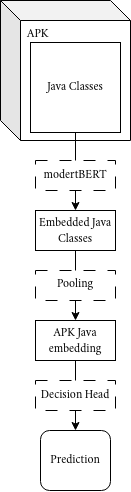
\includegraphics[width=0.6\marginparwidth]{4_Evaluation/java_transformer_schema.png}
    \caption{\label{fig:java_transformer_schema}
    Distribution of malware and goodware samples across datasets shown as pie charts.
    The datasets analyzed are ordered by size from largest to smallest.
    The number of APKs contained in the Dataset are shown in brackets}
\end{marginfigure}

% Intro
The last of the three variables in the proposed architecture \ref{fig:bertbased_malwaredetection_schema} is the decision head.
In the experiments conducted so far, the decision head was implemented as a simple fully connected layer 
trained to predict the label from the contextualized CLS embedding of the APK representation.
This approach has been quite effective. However, its applicability is limited.
When the tokenized APK representation exceeds the context window of the embedding model, 
the overall architecture becomes more complex.
If the representation cannot be summarized before embedding and exceed the context window, 
one way to maintain a transformer based embedding is to 
divide the representation into smaller chunks and embed them iteratively.
As a result, a single APK is no longer represented by one embedding but by multiple embeddings.
This poses a challenge, especially when the number of chunks varies between different APKs.
In such cases, training a unified decision head becomes difficult, as its input size can be 
both large and inconsistent.

% Pooling Idea
This issue can be addressed by pooling the embeddings into a smaller, fixed-size state.
When the representation varies in size, the number of viable pooling mechanisms decreases. 
However, there are still several possible approaches.
A simple pooling method is to compute statistical measures such as the minimum, maximum, or mean of the embeddings.
Since all embeddings share the same dimensionality, these measures can be calculated across each feature.
Another approach is to randomly select one of the embeddings as the final representation.

% Decision Head Experiment Setup
To assess the performance of different decision heads in embedding classification, another experiment was conducted.
While it keeps the general structure of the proposed architecture \ref{fig:bertbased_malwaredetection_schema}, 
it differs significantly from the previous setup shown in Figure \ref{fig:permission_transformer_schema}.
Figure \ref{fig:java_transformer_schema} illustrates the new experimental setup.
In this experiment, the representation of each APK is derived from the Java code that can be decompiled from the classes.dex file.
This Java code is then structured according to the corresponding classes.
This representation is quite extensive, as it consists of an average of 1,866 classes across the full 
transcending dataset as shown in figure \ref{fig:java_class_boxplots}.
This leads to a challenge for the base architecture \ref{fig:permission_transformer_schema}: 
in most cases, the APK representation exceeds the context window of the ModernBERT model, which is used to generate embeddings.
As discussed earlier, this requires breaking down the representation into smaller chunks.
For this purpose, Java classes were used as chunks.
While this method provides a straightforward way to segment the code, 
some individual Java classes still exceed the 8,000-token context window of ModernBERT.
When this occurred during the experiment, 
the Java class was processed iteratively using a sliding window approach with a stride of 6,000 tokens.
For these cases, the average of the CLS tokens generated during the sliding window process 
was used as the representation for the APK.
This approach ensured that each Java class was ultimately represented by a single CLS token.

\begin{margintable}[-5\baselineskip]
    \caption{\label{tab:matching_java_classes_transcend} Number of total java classes and classes that are mentioned by the manifest.xml file of the Transcending dataset. Also the number of classes that match by the classname is given}
    \footnotesize
    \begin{tabular*}{\linewidth}{@{\extracolsep{\fill}} lcr@{}}
        \toprule
        \textbf{Feature} & \textbf{Mean} & \textbf{Sum} \\
        \midrule
        Java Classes & 1866 & 483102763 \\
        Manifest Classes & 20 & 5277764 \\
        Matching Classes & 14 & 3791740 \\
        \bottomrule
    \end{tabular*}
\end{margintable}

% Match java classes with manifest file
One approach to reduce the number of Java classes requiring embedding was to process only those declared as activities, 
permissions, services, or receivers in the Manifest.xml file.
However, this method proved infeasible due to an obfuscation technique 
that altered the naming of Java classes in the manifest file.
A deeper analysis revealed that only 72\% of Java classes in the transcending dataset maintained 
a consistent naming convention between classes.dex and Manifest.xml (see Table \ref{tab:matching_java_classes_transcend}).
For the DexRay dataset, this percentage was even lower at just 12\% (see Table \ref{tab:matching_java_classes_dexray}),
this is consistent with the DexRay dataset explicitly focusing on including obfuscated APKs.
Due to this inconsistency, all Java classes within each APK had to be considered.

\begin{margintable}[-5\baselineskip]
    \caption{\label{tab:matching_java_classes_dexray} Number of total java classes and classes that are mentioned by the manifest.xml file of the DexRay dataset. Also the number of classes that match by the classname is given}
    \footnotesize
    \begin{tabular*}{\linewidth}{@{\extracolsep{\fill}} lcr@{}}
        \toprule
        \textbf{Feature} & \textbf{Mean} & \textbf{Sum} \\
        \midrule
        Java Classes & 1394 & 220838917 \\
        Manifest Classes & 58 & 9247905 \\
        Matching Classes & 7 & 1126716 \\
        \bottomrule
    \end{tabular*}
\end{margintable}

% Processing multiple Embeddings
As mentioned earlier, this approach results in a variable-sized embedding that needs to be classified.
To evaluate different decision heads, an experiment was conducted based on the method proposed in \cite{detectbert}.
In this setup, the detectBERT model is used as a decision head alongside three simpler approaches, 
and their performances are compared.
The alternative approaches are as follows:
Average: The mean of all Java class based CLS token embeddings is computed and processed by a fully connected layer.
The mean is calculated separately for each of the 768 features in the embedding vector, 
ensuring that the final mean embedding also has 768 features.
Addition: This follows the same process as the Average method but uses the sum instead 
of the mean to derive a single embedding representing the APK.
Random: One Java class is selected at random, and its CLS embedding is used to represent the APK for classification.

% Experiment description
Table \ref{tab:decision_head_comparison} presents the results of the experiment.
The performance of each decision head is assessed after training for 20 epochs on 
the same transcendence subset used in previous experiments.
To account for concept drift, this subset is split into training and test sets sequentially.

\begin{table}[b]
    \centering
    \caption{\label{tab:decision_head_comparison}Performance comparison of different decision heads on the Transcend dataset with a time-based split.}
    \resizebox{\textwidth}{!}{%
    \begin{tabular}{@{}lcccc@{}}
    \toprule
    \textbf{Decision Head} & \textbf{Accuracy} & \textbf{Precision} & \textbf{Recall} & \textbf{F1} \\ 
    \cmidrule(r){1-1} \cmidrule(lr){2-5}
    Average    & 83.00\% & 84.85\% & 80.35\% & 82.54\% \\
    Addition   & 59.15\% & 55.52\% & 92.00\% & 69.25\% \\
    DetectBERT & 74.28\% & 90.70\% & 54.10\% & 67.77\% \\
    Random     & 66.18\% & 67.13\% & 63.40\% & 65.21\% \\
    \bottomrule
    \end{tabular}%
    }
\end{table}

The average aggregation of CLS tokens achieved the best overall results, 
demonstrating high accuracy (83.00\%), precision (84.85\%), recall (80.35\%), 
and F1 score (82.54\%). This indicates balanced performance, 
effectively minimizing both false positives and false negatives.
The DetectBERT decision head showed moderate accuracy (74.28\%) 
and exceptionally high precision (90.7\%), but considerably lower recall (54.10\%). 
This indicates that while it rarely produces false positives, 
it frequently overlooks actual positives. 
The "Addition" decision head shows the highest recall (92.00\%) but low precision 
(55.52\%) and low accuracy (59.15\%). 
This approach is beneficial in applications where missing true positives is highly 
undesirable, even if it leads to many false positives. For example this could be useful 
for the task of identifying high risk APKs.
Lastly, the "Random" decision head serves as a baseline, 
performing modestly across all metrics (Accuracy: 66.18\%, Precision: 67.13\%, 
Recall: 63.40\%, F1: 65.21\%), 
highlighting the relative improvements of the other methods.
In terms of F1 score, both the Addition and DetectBERT approach perform only slightly better 
than the Random approach.
Overall the ranking of the four decision heads that are used is quite different from the 
performances reported on the smali embeddings by \cite{detectbert}, which does seem to 
overestimate the performance of DetectBERT.

In the chapter \ref{sec:detectbert} we evaluated the DetectBERT decision head on the same 
dataset with the same split but on smali based embeddings calculated by dexBERT rather 
than java based embeddings calculate by ModernBERT. 
The DetectBERT head achieved improved performance on these embeddings, 
obtaining an accuracy of 80.13\%, precision of 80.91\%, recall of 78.88\%, and an F1-score of 79.88\% 
as shown in table \ref{tab:detectbert-results}.
Compared to the Java based embeddings, this indicates that DetectBERT performs significantly better 
with smali based embeddings, especially regarding recall, 
indicating that the choice of the decision head does depend on the type of embedding that is used.

The decreased effectiveness of the DetectBERT decision when comparing our results with the results 
reported by DetectBERT (97\% F1 score; table \ref{tab:detectbert_performance_original}) might be explained 
by the dataset that has been used. While the transcend subset that we used seems to be an easier benchmark 
than the full trancend dataset, it was balanced on the amount of smali and java classes between labels.
If DetectBERT works similarly to the aggregation head, in a sense that the amount of classes 
that are embedded have a direct impact on the prediction derived, this drop can be explained.
We showed in chapter \ref{sec:datasets} that the dexRay dataset, that was used for the experiments that 
led to the 97\% F1 score, is highly imbalanced in terms of smali classes between labels as visualized by the 
boxplot in figure \ref{fig:smali_class_boxplots}.

